% last updated in April 2002 by Antje Endemann
% Based on CVPR 07 and LNCS, with modifications by DAF, AZ and elle, 2008 and AA, 2010, and CC, 2011; TT, 2014

\documentclass[runningheads]{llncs}
\usepackage{graphicx}
\usepackage{amsmath,amssymb} % define this before the line numbering.
\usepackage{ruler}
\usepackage{color}
\usepackage{array}
\usepackage{float}
\usepackage{subfig,caption}
%\usepackage{subcaption}
\usepackage{comment}
\usepackage[width=122mm,left=12mm,paperwidth=146mm,height=193mm,top=12mm,paperheight=217mm]{geometry}
\begin{document}
% \renewcommand\thelinenumber{\color[rgb]{0.2,0.5,0.8}\normalfont\sffamily\scriptsize\arabic{linenumber}\color[rgb]{0,0,0}}
% \renewcommand\makeLineNumber {\hss\thelinenumber\ \hspace{6mm} \rlap{\hskip\textwidth\ \hspace{6.5mm}\thelinenumber}}
% \linenumbers
\pagestyle{headings}
\mainmatter
\def\ECCV14SubNumber{***}  % Insert your submission number here

\title{Author Guidelines for ECCV Submission} % Replace with your title

\titlerunning{ECCV-14 submission ID \ECCV14SubNumber}

\authorrunning{ECCV-14 submission ID \ECCV14SubNumber}

\author{Anonymous ECCV submission}
\institute{Paper ID \ECCV14SubNumber}


\maketitle

\begin{abstract}

\end{abstract}


\section{Introduction}
Features learnt by a large-scale convolutional neural network trained for the task of image classification on the Imagenet challenge have been used to achieve impressive results on different computer vision tasks. Since, these networks are high capacity learners they cannot be trained on small data sets. Consequently, in their recent work ..have used fine-tuning to improve performance. For example, (\cite RCNN) used fine-tuning to boost performance on pascal detection challenge by nearly 25 \% (relative) mean ap points over the performance of an un-tuned network.

Fine-tuning a network essentially involves starting from a set of pre-learned parameters and slowly updating them to minimize a target loss function. Till date, there has been little work looking at the effect of fine-tuning on various layers of a discriminatively trained convolutional neural network. In this work, we address this question. Our findings indicate that during finetuning most of the learning takes place in the top 2 fully connected layers whereas the convolutional layers are largely un-changed. We quantify this claim by first comparing entropy of filters before and after fine-tuning. Secondly, we demonstrate that keeping layers 1-5 fixed while fine-tuning leads to negligible decrease in performance. Next, we show pool-5 features can be treated as generic feature extractor on top of which non-linear classifiers can be used to achieve good results. For developing a scientific understanding of how the network trains, we analyse conv-nets trained for different number of iterations. We find that most of the learning happens quite early on and that the network naturally learns in a layer-wise fashion. Finally, we conclude by providing some insights into how important is the magnitude of feature activation, the location and so on. 

This suggests, that layers 1-5 can be treated as a generic feature extraction engine which can serve as a starting point for other computer vision models. Reduce time for fine-tuning. 
The most commonly used conv-net architecture, first proposed by Kr consists of 5 convolutional layers followed by 2 fully connected layer. 
 
Inspite of the impressive performance, the question of how information is represented and what various layers are encoding is unclear. 

Some recent work has focussed on coming up with visualization techniques to analyze and understand the tuning properties of filters in different layers. Although, visually impressive its hard to draw meaningful conclusions about properties of filters in different layers. We start of f with a detailed analysis of how good are different layers for image classification. We provide an entropy analysis ...

Next, we try to answer how much information is encoded by the activity of individual filters and how important is the spatial location of where the filters activate.      

Next, we show that the network trains layer-wise and the convolutional layers are well formed quite early into the training. 

Next, we argue that fine-tuning majorly effects the final two layers and that layers 1-5 can be treated as a generic feature extractor. This allows us a moderate speed-up in training time. 

\section{Method}
\subsection{Network-Architecture}
For all our experiments we closely follow the architecture proposed in \cite{alex}. The first 2 layers consist of 4 sublayers each - convolution (conv), followed by rectified linear units (relu), pooling (pool) and contrast normalization (norm). Layers 3, 4 are composed of convolutional units followed by relu units. Layer 5 consists of convolutional units, followed by relu and pooling. The last two layers are fully connected (fc). In this work when we refer to a layer without referring to a particular sub-layer - then for layer 1,2,5 we mean the output of the pooling stage and for layers 3,4,6,7 we mean the output of relu units.

\subsection{Training Conv-Nets}
\label{sub:train}
We have trained all our models using the publically available code \cite{caffe} and Nvidia K40 GPUs. Our imagenet network was trained for 310000 iterations and achieves an error rate only about 2\% higher on the ILSVRC validation set 2012. We refer to this network as the Alex-net .

\subsection{Fine-Tuning}
\label{sub:fine-train}
For a particular task, we fine-tune conv-nets by running SGD (Stochastic Gradient) with a starting learning rate set to $\frac{1}{10}^{th}$ of the intial learning rate of the imagenet model. This choice has been made because we donot want to drastically change the parameters of the network and overfit to the training set. At every 20,000 iterations we reduce the learning rate by a factor of 10 and use a mini-batch size of 128.

\subsubsection{Fine-Tuning for PASCAL}: Closely following the work of \cite{rcnn} we use region proposals generated by selective search algorithm for fine-tuning. Each region is warped to a size of 227*227*3. Regions with IOU (intersection over union) $\geq$ 0.5 with ground truth bounding boxes are treated as positives and rest as negatives. This  results into a 21-way classification problem (20 PASCAL classes + background). We tuned this network for 70000 iterations and refer to it as the FT network in the sections below.

**To-DO ? Specify the procees of fc-only fine-tuning.  ***

\section{How does fine-tuning effect the network ?}



\subsection{Discriminative Fine Tuning Helps}
**To-Do** Results on SUN



\subsection{How does the entropy of filters vary in the network ?}
Units become more specific - but entropy of individual units - doesnt really increases until one reaches layer 6. (Ground Truth Bounding Box.) Put the picture below without the fine-tuned network.


In order to estimate the entropy, for all ground truth bounding boxes, we compute activations of each filter (both in fully-connected and convloutional layers). With each activation value we associate the class-label of the bounding box. Next, we sort the scores in decreasing order and compute entropy of the histogram counts of classes at 100 equally spaced thresholds. The area under this curve is used as a measure of entropy. 

(Contrast to mid-level patches idea - where greedily select filters based on entropy). 

\begin{figure}
\centering
\subfloat{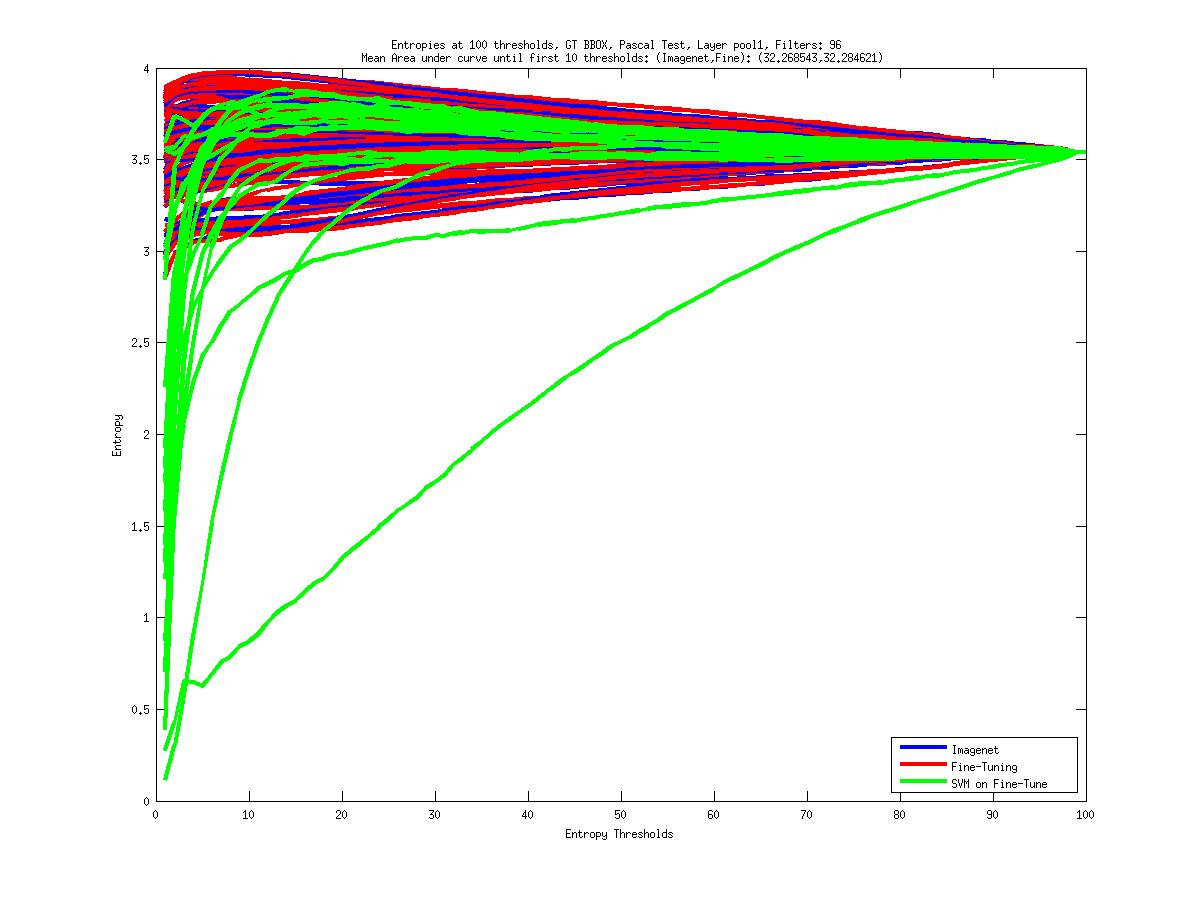
\includegraphics[scale=0.15]{images/pool1_th100_plot.jpg}}
\subfloat{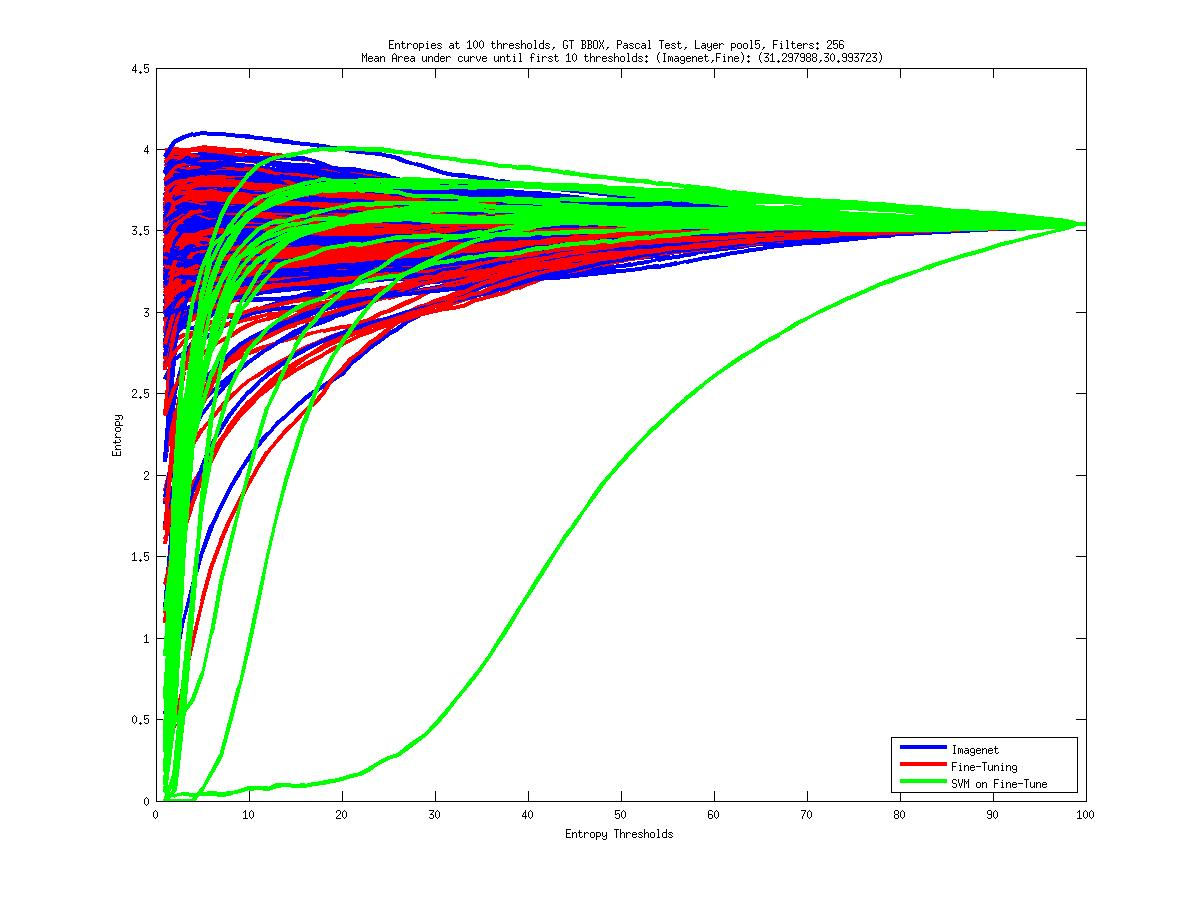
\includegraphics[scale=0.15]{images/pool5_th100_plot.jpg}} \\
\subfloat{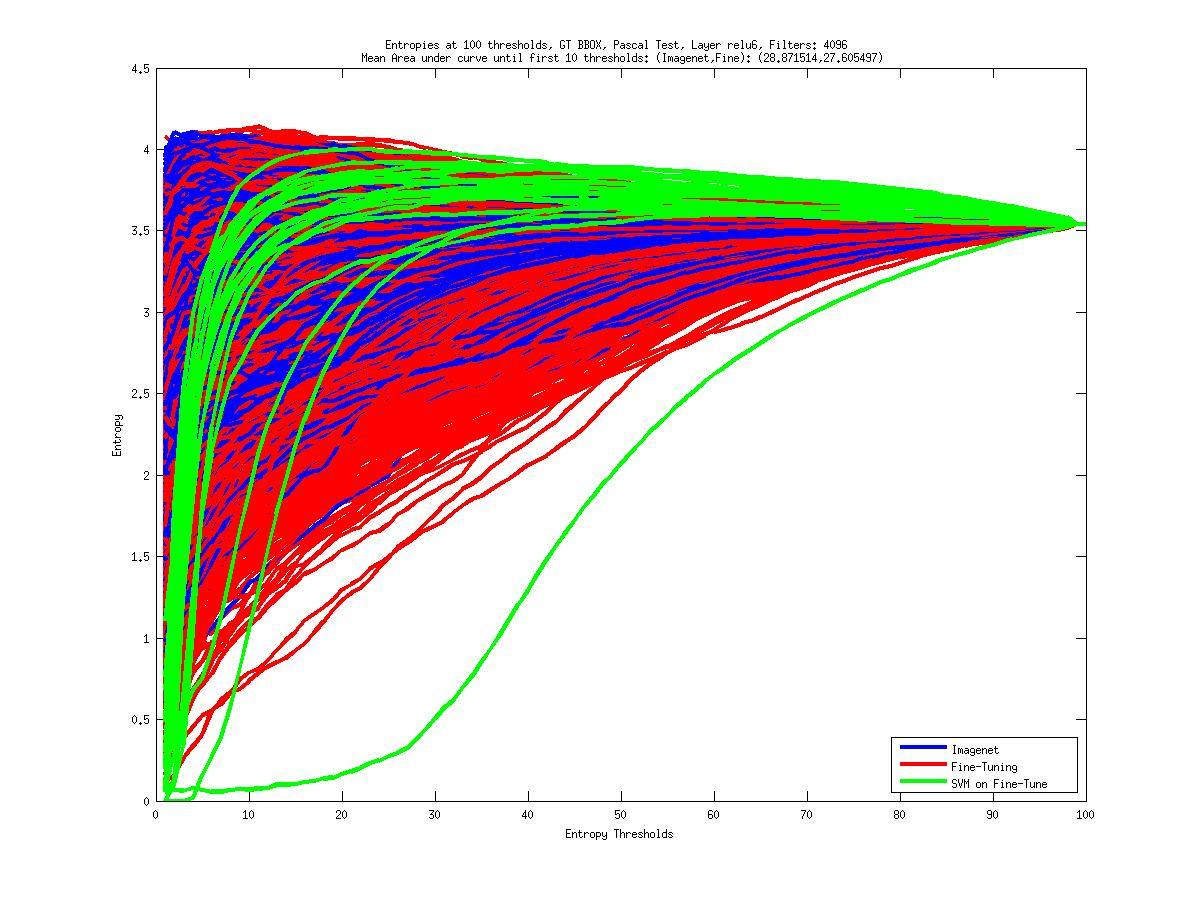
\includegraphics[scale=0.15]{images/relu6_th100_plot.jpg}} 
\subfloat{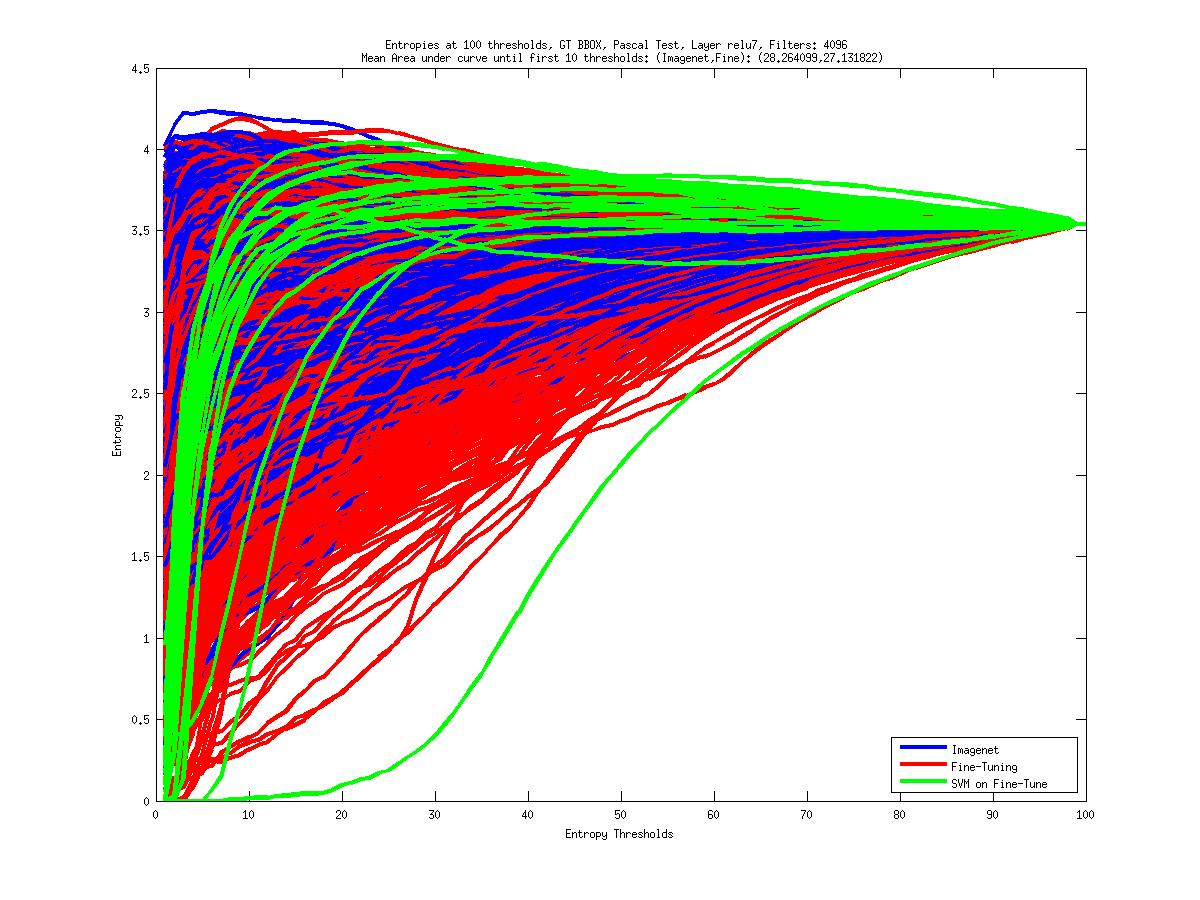
\includegraphics[scale=0.15]{images/relu7_th100_plot.jpg}}
\caption{Entropy filters at various layers.}
\label{fig:example}
\end{figure}


\begin{figure}[H]
\centering
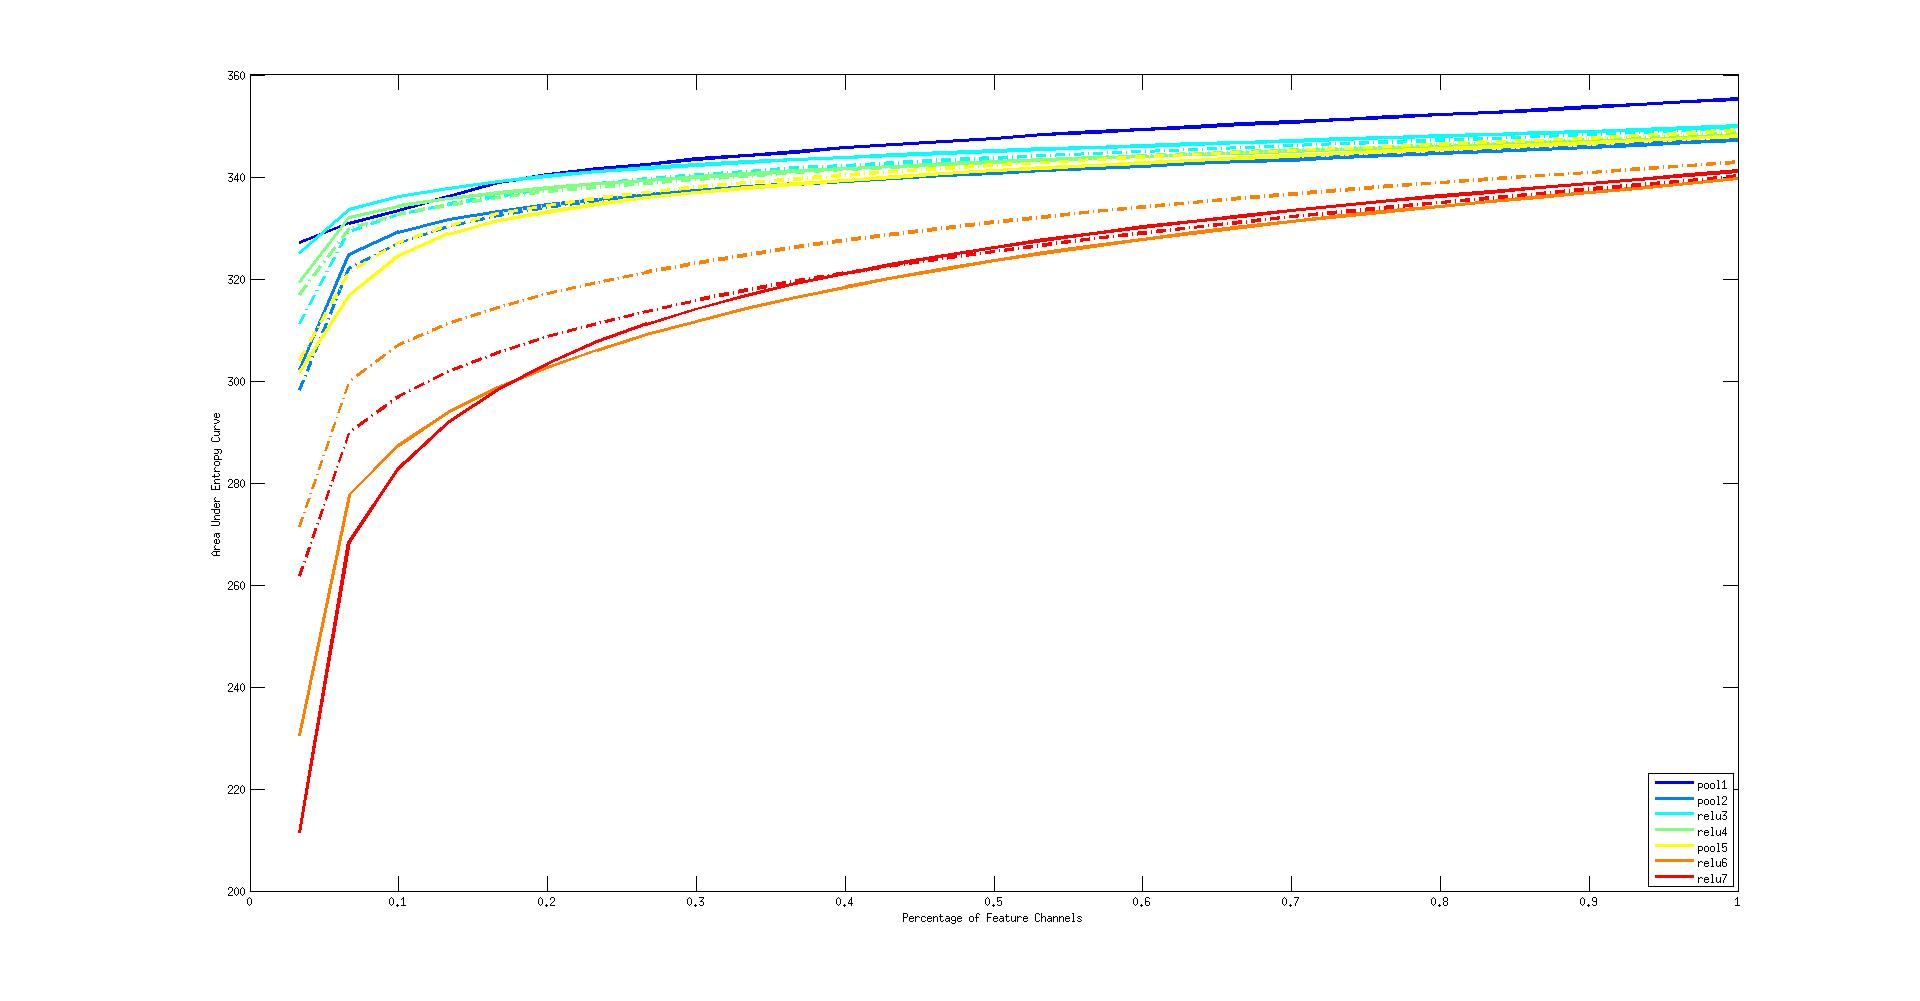
\includegraphics[height=6.5cm]{images/entropy_layers.jpg}
\caption{The plot shows the variation in entropy of different layers of a convolutional network trained on imagenet (dot-dash line) and a network fine-tuned for object detection on PASCAL dataset.}
\label{fig:example}
\end{figure}





\setlength{\tabcolsep}{2pt}
\begin{table}
\begin{center}
\caption{Effect of fine-tuning a network for 3 tasks in the PASCAL VOC-2007 Challenge}
\label{table:fine-effect}
\begin{tabular}{l|ccc|ccc|ccc}
\hline\noalign{\smallskip}
Layer & \multicolumn{3}{c}{Image Classification}  & \multicolumn{3}{c}{GT Box Classification} & \multicolumn{3}{c}{Detection} \\
\hline
      & alex-net & fc-tune & all-tune & alex-net & fc-tune & all-tune & alex-net & fc-tune & all-tune \\
\hline
pool-5   & 65.6 & & 64.6 & 79.1 & 79.1 & 79.5 & 45.0 & 45.0 & 47.6 \\
relu-6   & 70.6 & & 71.7 & 79.4 & 82.0 & 82.3 &  - & 51.0 & 53.1  \\
relu-7   & 73.6 & & 73.2 & 79.9 & 83.4 & 85.2  & 45.5 & 53.3 & 54.1 \\
\hline
\end{tabular}
\end{center}
\end{table}
\setlength{\tabcolsep}{1.4pt}


\setlength{\tabcolsep}{4pt}
\begin{table}
\begin{center}
\caption{Layerwise effect of fine-tuning, GT-bbox classification, FT: Fine-Tuned, C-Net: Caffe-Net}
\label{table:headings}
\begin{tabular}{ccc|ccc|ccc|ccc}
\hline\noalign{\smallskip}
Layer & C-Net & FT & Layer & C-Net & FT & Layer & C-Net & FT & Layer & C-Net & FT \\
\noalign{\smallskip}
\hline
\noalign{\smallskip}
l1 & 43.2 & 43.2 & l3 & 73.3 & 73.7 & l5 & 79.1 & 79.5 & \textbf{l7} & \textbf{79.9} & \textbf{85.1} \\
l2 & 67.1 & 67.7 & l4 & 75.5 & 77.8 & \textbf{l6} & \textbf{79.4} & \textbf{82.3} \\
\hline
\end{tabular}
\end{center}
\end{table}
\setlength{\tabcolsep}{1.4pt}

**To-Do**: Difference in Entropy


\subsection{FC-Only Fine-Tuning is Sufficient}
We evaluated 3 convolutional neural networks (namely caffe-net, FT and FC-FT) on the tasks of image classification, ground truth bounding box classification and detection. The results can be seen in table \ref{table:fine-effect}. The mean-AP on the tasks of ground truth bounding box classification and detection increases, whereas performance is uneffected for the task of classification. The performance of the network with tuning the fully connected layers is comparable to the performance of


In order to test our hypothesis that bulk of the learning required for good performance on a new task happens in the fully connected (FC) layers - we finetune caffe-net in two ways. In the first method, we set the learning rate for all the convolutional layers to be zero and randomly intialize the fully connected layers. The second network has non-zero learning rates for all the layers and the FC-layer parameters are initialized to their values in a conv-net trained on imagenet. Fine-tuning is performed  using the selective search bounding box proposals (\cite{rcnn}). The ground truth bounding boxes are assigned their respective class labels whereas any region with less than 0.3 IOU with a ground truth bounding box is assigned to background class. We fine-tune both the networks for 70,000 iterations.

Results of this experiment are presented in table \ref{table:det-fine}. The full fine-tuned network does slightly better when we train a detector on pool-5 features but the performance after layer 7 is almost equal. 

\setlength{\tabcolsep}{1pt}
\begin{table}
\begin{center}
\caption{Detection: Fine-Tuning Effects.}
\label{table:det-fine}
\tiny
\begin{tabular}{l|cccccccccccccccccccc||c}
\hline\noalign{\smallskip}
Feature & aero & bike & bird & boat & bottle & bus & car & cat & chair & cow & table & dog & horse & mbike & person & plant & sheep & sofa & train & tv & mAP \\
\noalign{\smallskip}
\hline
l5 & 51.9 & 61.1 & 36.8 & 28.4 & 23.7 & 52.3 & 60.8 & 48.4 & 24.9 & 47.1 & 47.5 & 42.1 & 55.6 & 58.7 & 42.5 & 24.5 & 46.9 & 39.3 & 52.0 & 55.4 & 45.0 \\
l5-ft & 57.8 & 63.9 & 38.8 & 28.0 & 29.0&54.8&66.9&51.3 & 30.5 & 52.1 & 45.2 & 43.2 & 57.3 & 58.8 & 46.0 & 27.2 & 51.2 & 39.3 & 53.3 & 56.6 & 47.6 \\
\hline 
l6-ft &63.5 & 66.3 & 48.7 & 38.1 & 30.6 & 61.4 & 70.9 & 60.3 & 34.8 & 57.8 & 47.6 & 53.6 & 59.8 & 63.5 & 52.5 & 29.8 & 54.6 & 48.2 & 58.5 & 62.2 & 53.1 \\
l6-fc-ft& 61.4 & 63.9 & 44.2 & 36.2 & 29.0 & 59.9 & 66.0 & 55.3 & 31.1 & 57.6 & 49.5 & 49.4 & 59.4 & 63.7 & 50.8 & 29.5 & 54.1 & 43.2 & 57.4 & 58.8 & 51.0 \\
\hline
l7 & 57.6 & 57.2 & 41.4 & 31.2 & 25.6 & 52.4 & 58.8 & 50.9 & 25.2 & 50.4 & 42.7 & 47.1 & 52.2 & 55.6 & 44.5 & 23.9 & 48.0 & 38.1 & 51.5 & 56.6 & 45.5 \\
l7-ft & 64.3 & 69.6 & 50.1 & 41.8 & 32.0 & 62.6 & 71.0 & 60.6 & 32.8 & 58.5 & 46.4 & 56.0 & 60.0 & 66.9 & 54.2 & 31.5 & 52.7 & 48.8 & 57.7 & 64.7 & 54.1 \\
l7-fc-ft & 62.9 & 65.2 & 47.5 & 39.0 & 30.3 & 63.1 & 68.4 & 59.7 & 34.2 & 58.5 & 52.0 & 53.8 & 60.7 & 65.3 & 53.0 & 30.2 & 55.5 & 46.3 & 57.7 & 62.2 & 53.3 \\
\noalign{\smallskip}
\hline
\end{tabular}
\end{center}
\end{table}
\setlength{\tabcolsep}{1.4pt}


The performance of the FC-FT network at layer 5 is slighly worse by 2.6 points, but at layer 7 this difference is only 0.8 points. 

Next, we compare the performance of both the networks for the task of classifying ground-truth bounding boxes from PASCAL-VOC-2007 challenge.  

\subsection{Replacing fc-layers by other-non linear classifiers}
**Stacked Kernel Results ***



\section{Where is the information - location or magnitude?}
Understanding how information is encoded across layers of the convolutional neural network is an important question. In this section we focus on answering the following two questions:
\begin{itemize}
\item How important is the location where a filter fires?
\item How much information is contained in the magnitude of filter activations?
\end{itemize}

We answer these questions using a set of carefully designed ablation studies. The difference between the baseline performance obtained by using vectorized  layer (i.e. i.e. "unrolling" a layer of size $sz \times sz \times nf$ into a 1 dimensional vector) and an ablated feature vector is used as a measure of importance for factors under study. In all our experiments in this section, we train linear svms for evaluation.

\begin{figure}[H]
\centering
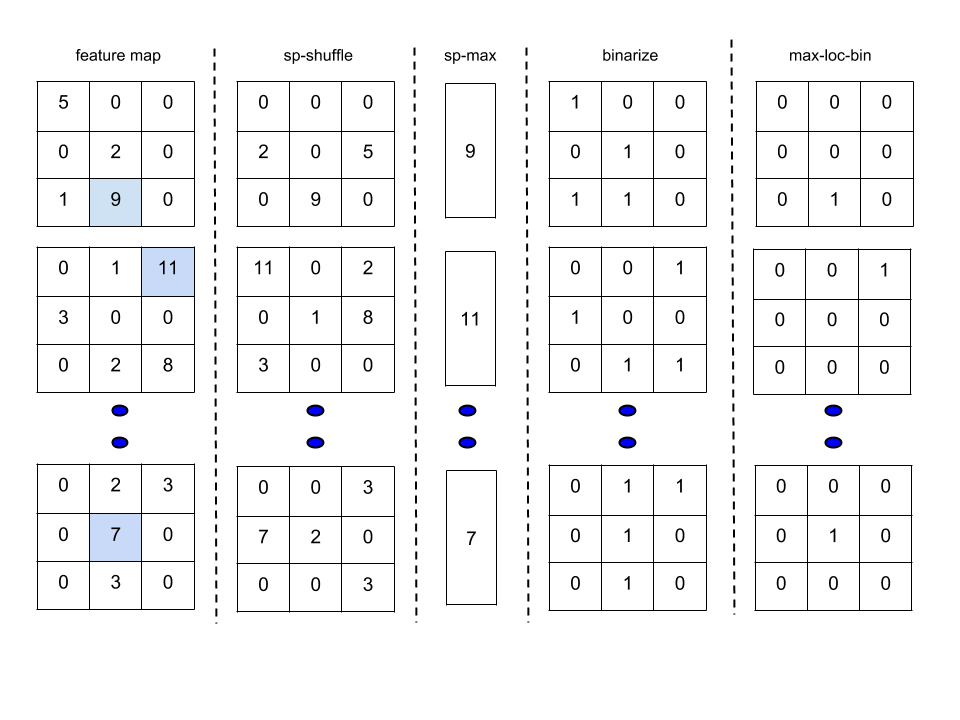
\includegraphics[height=6.5cm]{images/features.png}
\caption{Different feature ablations used in analysis described in sec. \ref{sub:imp-loc}, \ref{sub:imp-mag}. For the purpose of illustration, consider each 3*3 block in first column as a feature map. The second column shows \textit{spatial-shuffle}, i.e. the  result of applying an independent spatial random permutation to each feature map. Third column depicts \textit{spatial max}, i.e. selecting the max activation in each featue map. Fourth column illustrates \textit{binarization} whereas the last column selects the maximum value in each feature map, binarizes it but also retains the location where the filter fired.}
\label{fig:features}
\end{figure}

\subsection{How important is where a filter activates?}
\label{sub:imp-loc}
In the first ablation experiment we 



\setlength{\tabcolsep}{1pt}
\begin{table}
\begin{center}
\caption{Detection: Effect of various feature transformations.}
\label{table:headings}
\tiny
\begin{tabular}{l|cccccccccccccccccccc||c}
\hline\noalign{\smallskip}
Feature & aero & bike & bird & boat & bottle & bus & car & cat & chair & cow & table & dog & horse & mbike & person & plant & sheep & sofa & train & tv & mAP \\
\noalign{\smallskip}
\hline
spMax & 35.0 & 38.7 & 17.3 & 16.9 & 13.9 & 38.4 & 45.6 & 29.2 & 11.0 & 20.2 & 21.0 & 23.5 & 27.2 & 37.0 & 20.5 & 7.0 & 30.3 & 13.4 & 28.3 & 32.9 & 25.4 \\
sm-bn-lc & 49.1 & 48.0 & 19.0 & 15.2 & 12.9 & 44.7 & 57.0 & 32.8 & 11.9 & 32.5 & 19.0 & 25.0 & 37.5 & 41.6 & 34.8 & 15.6 & 34.1 & 13.0 & 35.7 & 44.9 & 31.2 \\
crop-1 & 48.2 & 59.8 & 32.2 & 20.0 & 24.6 & 46.2 & 61.2 & 41.6 & 20.6 & 46.3 & 32.9 & 38.6 & 49.9 & 53.1 & 41.8 & 25.1 & 45.0 & 23.8 & 46.2 & 51.7 & 40.4 \\
binary & 57.9 & 61.3 & 32.6 & 24.7 & 27.5 & 55.0 & 64.7 & 49.8 & 25.3 & 47.4 & 44.5 & 40.3 & 54.6 & 56.4 & 43.6 & 27.1 & 48.4 & 41.6 & 54.3 & 57.6 & 45.7 \\
pool-5  & 57.8 & 63.9 & 38.8 & 28.0 & 29.0 & 54.8 & 66.9 & 51.3 & 30.5 & 52.1 & 45.2 & 43.2 & 57.3 & 58.8 & 46.0 & 27.2 & 51.2 & 39.3 & 53.3 & 56.6 & 47.6 \\
\noalign{\smallskip}
\hline
\end{tabular}
\end{center}
\end{table}
\setlength{\tabcolsep}{1.4pt}




\setlength{\tabcolsep}{4pt}
\begin{table}
\begin{center}
\caption{Mean AP on PASCAL-VOC 2007 Classification}
\label{table:headings}
\begin{tabular}{lccccc}
\hline\noalign{\smallskip}
Layer Name & Unroll & Spatial-Shuffle & Spatial-Max & Binarize & Binarize+Loc\\
\noalign{\smallskip}
\hline
\noalign{\smallskip}
pool-1 & 25.1 & 15.0 & 19.5 & 25.4 \\
pool-2 & 44.9 & 33.5 & 40.2 & 43.0\\
conv-3 & 50.1 & 40.4 & 54.2 & 47.0\\
conv-4 & 54.2 & 45.3 & 57.0 & 51.3\\
pool-5 & 65.6 & 59.6 & 62.6 & 60.5\\
relu-6 & 70.6 &  -   &  -   & 71.4 \\
relu-7 & 73.6 &  -   &  -   & 74.1 \\
\hline
\end{tabular}
\end{center}
\end{table}
\setlength{\tabcolsep}{1.4pt}


\subsection{How important is the magnitude of activation ?}
\label{sub:imp-mag}





\section{How common are Grand-Mother like Units ?}
How information is represented in deep architectures such as convolutional neural networks is an open question. We know that the first layer ends up learning gabor like edge detectors and that units in the final layers are very class specific. However, we are far from understanding the representations learned in the middle layers. Developing this understanding is crucial in order to effectively devise methods capable of fully exploiting the rich feature hierarchy provided by convolutional networks.

Some recent work addressing this question has focussed on developing visualization techniques (zeiler, simoyan, google paper) to understand feature tuning of different filters. \cite{zeiler} presented a deconvolution strategy which effectively uses backprojection to find image regions which cause a particular filter to activate.  \cite{simoyan} on the other hand pose tuning as an optimization problem and try to estimate optimal stimuli for a given unit in the higher layers. \cite{google} train a massive non-convolutional network and show the presence of cat and people specific units learnt by their network. We feel that although visualizations are helpful they donot convey the full story. More-over they are subjective and it is unclear what conclusions one might draw. In particular, finding a few units tuned to people or cats tells us very little about what other units might be doing. To best of our knowledge there is no work which tries to objectively answer this question.

Also, most of such work can be treated as different interpretations of estimating/understanding P(Activation of a single unit | Class). Although this is linked to P(Class | Activation) via Bayes theorem it is hard to emperically estimate P(Class). More often than not our goal is to use to features for task of prediction. With this motivation we believe that P(Class | Activation) is also an important metric to study. One more way of looking at these metrics is the whether we are more interested to probe invariance of a particular filter or we are interested in understanding the discriminative power which it provides. A filter can be both highly invariant and very discrminative or higly invariant and very generic.  

**Information theoretic arguments ?? ** 

Aprioiri it is unclear whether discriminative information about a certain class is encoded in distribution of a group of filter activations or whether there are specific units tuned to specific classes. From the principles of efficient coding (such as Hoffman encoding) - an optimal code (Redundancy vs ...)

The question we pose is whether the representation learned by a deep conv-net consist of many "grand-mother cells" (specifically tuned units for various classes) or whether it is necessary to consider the distribution of activations across many filters to infer any semantics about the image. We develop two methods presented in the following subsections in an attempt to objectively answer this question.


A lot of recent (...) has focussed on understanding the invariance properties of each filter. In particular, in one form or the other they have focussed on estimating $P(Activation | Class)$. [simoyan and google] explicitly maximize this metric to find the optimal input for a unit. zeiler et al on the other hand start off with a specific image and use it for deconvolution. If a prioiri, we knew that information representation is not distributed and a very few neurons are necessary to represent a certain class - studying the invariance is the correct thing to do. However, if we believe that information is distributed - then we can have a group of filters wherein each filter by itself may not be tuned for a particular class but the activation of group of filters 

\subsection{Finding class specific units}
\label{sub:class-specific-unit}
In order to study the tuning properties of various units, for each PASCAL class we emperically estimate P(Class | Activation of unit > threshold) for all 256 filters in layer 5. For this purpose, we restrict ourselves to ground truth bounding boxes in contrast to full images as a single image may contain multiple objects and thereby confound any interpretations drawn from our analysis. 

Each filter in Pool-5 layer appears as $6 \times 6$ spatial map. Thus for each ground truth bounding box we get 36 activation samples for a particular unit. Given, N boxes we end up with 36N samples for each filter. For each filter, we sort the activations values and use this to compute the probability of a unit representing a class given its value is more than some threshold. We compute this probability for 1000 thr

From our analysis, we find that in order to predict the category of a given image, neither the magnitude nor the location of where filters activate is critical. On the other hand, 


As described in section .. we compute the entropy of each filter in the fifth layer of the network. Next, we rank all the filters by their entropy. At pool-5, each image produces a $6 \times 6 \times 256 $ feature vector (256 filter maps of size $6 \times 6$). For each filter map - we select the maximum activation which results into a 256-dimensional vector. Now, we train SVM 
 
For tasks of image classification, bounding box classification - position doesnot really matter. 

\subsection{How many units do we need?}
\label{sub:how-many}
The tuning analysis presented in section \ref{sub:class-specific-unit} is not sufficient by itself to answer how many units are needed in order to classify a given image. This is because, there might be important information in simultaneous firing of a group of filters which is ignored while looking only at individual filters. 

Consequently, in order to answer the above posed question we train linear a svm for each class using only a subset of 256 pool-5 filters. In particular we construct subsets of size k, where k takes the values - [1,2,3,5,10,15,20,25,30,35,40,45, \newline 50,80, 100,128,256]. A subset of size k is constucted independently for each class using a greedy selection strategy described in figure \ref{fig:sel-strategy}. We use the variation in performance with the number of filters needed as a metric to evaluate how many filters are needed for each class. 
  
\begin{figure}[H]
\centering
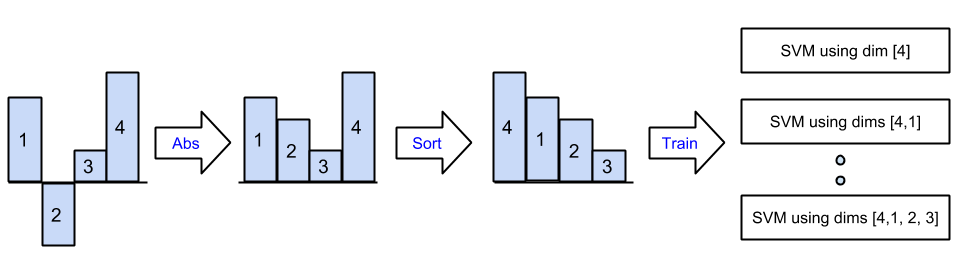
\includegraphics[scale=0.30]{images/how-many.png}
\caption{Illustration of our greedy strategy for constructing subsets of filters. For each class we first train a linear-svm using the spatial-max feature transformation described in section \ref{sub:imp-loc}. Spatial-max leaves us with a 256-D vector wherein each dimension has a one to one correspondence with 256 pool-5 filters. We use the magnitude of each dimension of the learnt weight vector as a proxy for the importance of that dimension towards discriminating a given class. For the purpose of illustration we describe the procedure with a 4-D weight vector shown on the extreme left (the numbers on each bar are the "dimension"). Firstly, we take the absolute value for each dimension and then sort the dimensions based on this value. Then, we chose the top k filters/dimensions from this ranked list to construct a subset of size k.}
\label{fig:sel-strategy}
\end{figure}

The results of our analysis are summarized in fig \ref{fig:svm-sel-dims} and table \ref{table:num-fil}. For classes such as persons, cars, cats we require a relatively few number of filters, but for most of the classes we need to look at around 30-40 filters to achieve atleast 90\% of the full performance. This also indicates, that for a few classes yes, there are grand-mother kind of neurons but for a lot of classes the representation is distributed. Also, as expected the fine-tuned network requires activations of a fewer numbers of filters to achieve the same performance but this reduction in number of filters is not large. 

\begin{figure}[H]
\centering
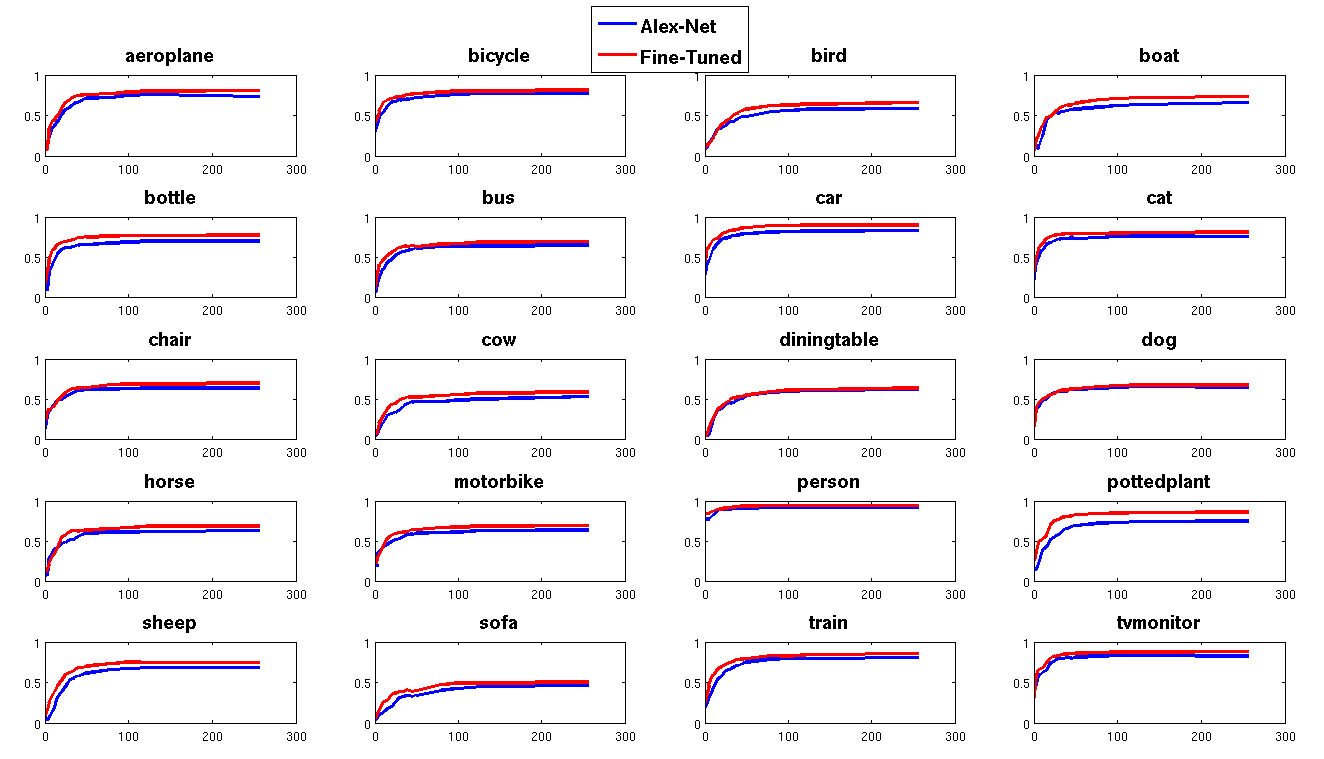
\includegraphics[height=6.5cm]{images/svm_seldims.png}
\caption{Analysis of how many filters are required to classify ground truth bounding boxes for 20 categories taken from PASCAL-2007 detection challenge. The y-axis in each of plot represents classification accuracy measured as mean-ap where as x-axis stand for the number of filters.)}
\label{fig:svm-sel-dims}
\end{figure}



\setlength{\tabcolsep}{1pt}
\begin{table}
\begin{center}
\caption{Number of filters required to achieve 50\% ,90\% of the full performance for PASCAL classes using Alex-Net(AN) and the Fine-Tuned network(FT)}
\label{table:num-fil}
\tiny
\begin{tabular}{lc||cccccccccccccccccccc}
\hline\noalign{\smallskip}
Net & AP & aero & bike & bird & boat & bottle & bus & car & cat & chair & cow & table & dog & horse & mbike & person & plant & sheep & sofa & train & tv \\
\noalign{\smallskip}
\hline
AN & 50 & 15 & 3 & 15 & 15 & 10 & 10 & 3 & 2 & 5 & 15 & 15 & 2 & 10 & 3 & 1 & 10 & 20 & 25 & 10 & 2 \\ 
FT & 50 & 10 & 1 & 20 & 15 & 5 & 5 & 2 & 2 & 3 & 10 & 15 & 3 & 15 & 10 & 1 & 5 & 15 & 15 & 5 & 2 \\
\hline
\noalign{\smallskip}
AN & 90 & 40 & 35 & 80 & 80 & 35 & 40 & 30 & 20 & 35 & 100 & 80 & 30 & 45 & 40 & 15 & 45 & 50 & 100 & 45 & 25 \\
FT & 90 & 35 & 30 & 80 & 80 & 30 & 35 & 25 & 20 & 35 & 50 & 80 & 35 & 30 & 40 & 10 & 35 & 40 & 80 & 40 & 20 \\
\hline
\end{tabular}
\end{center}
\end{table}
\setlength{\tabcolsep}{1.4pt}


\section{Can we speed things up?}
Convolutional neural networks take a long time to train. For achieving state of art accuracy on the imagenet challenge these networks are often trained on high-end GPUs for more than 7 days. Even our implementation of fine-tuning following the approach proposed in \cite{rcnn} takes more than 12 hours on a Nvidia Tesla-K40. A way to speed up training will allow for a rich exploration of network architectures and parameters which is currently not possible.    

As a first step towards addressing this problem, we looked at the evolution of training loss and validation accuracy as the training progresses (fig \ref{fig:conv1}.) The top-1 accuracy on the imagenet validation set at 15K iterations is at 29.5 \% and 38.13\% at 50K iterations (compared to 57.4 \% at 310K iterations). The training loss rapidly increases initially and then there is a slow sluggish decay except for the point where learning rate is decimated by a factor of 10 at 100K iterations.

\begin{figure}
\centering
\subfloat{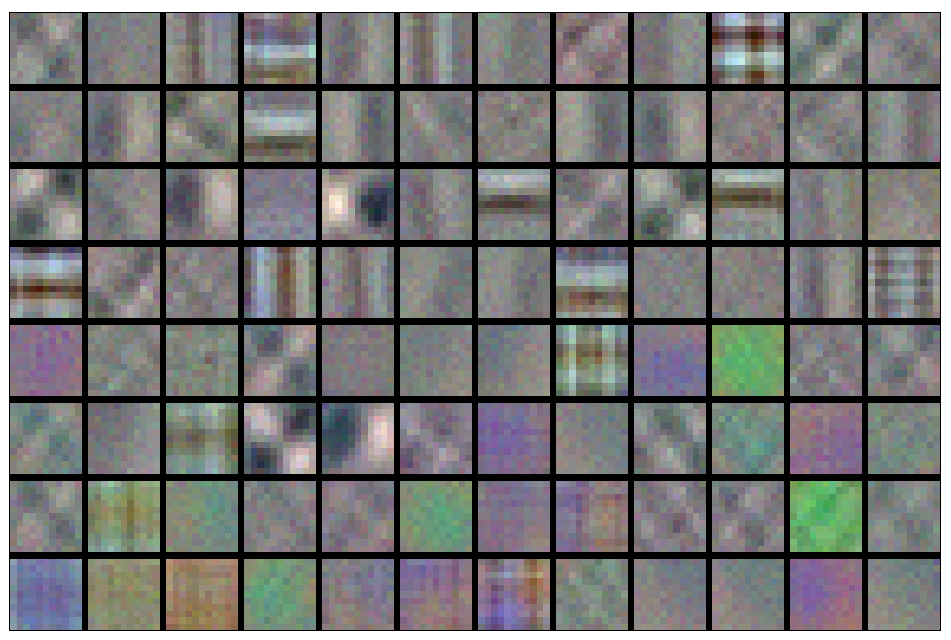
\includegraphics[scale=0.10]{images/l1_filters_iter5000.png}} \hspace{2mm}
\subfloat{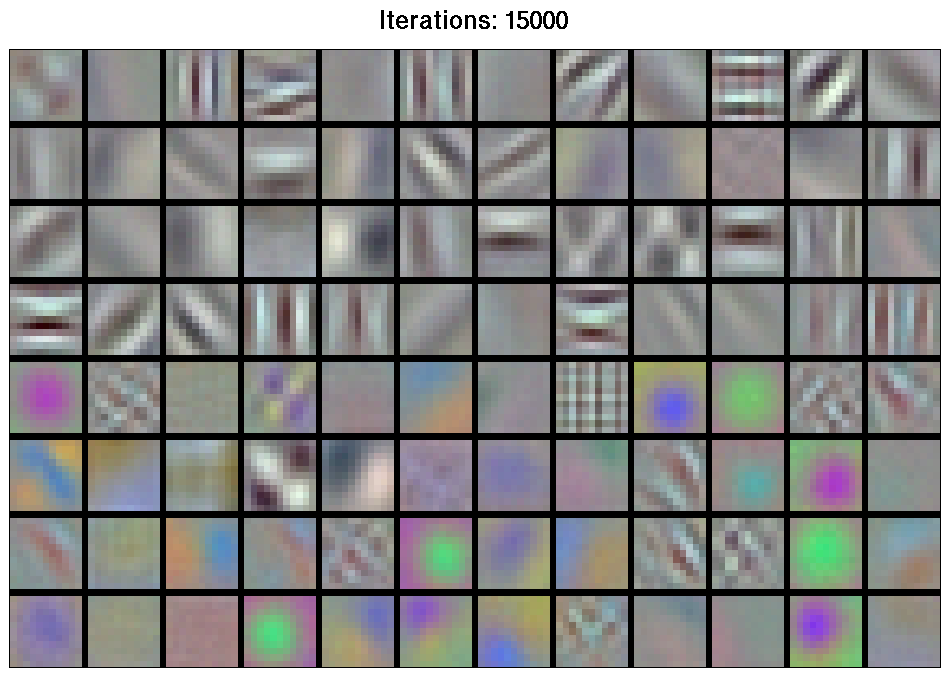
\includegraphics[scale=0.10]{images/l1_filters_iter15000.png}} \hspace{2mm}
\subfloat{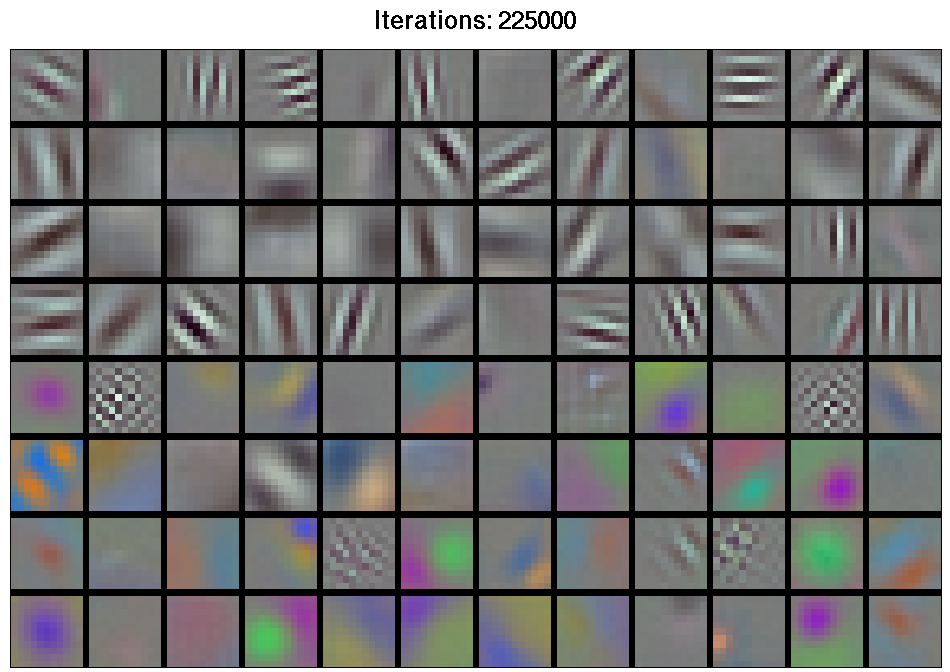
\includegraphics[scale=0.10]{images/l1_filters_iter225000.png}} \\
\subfloat{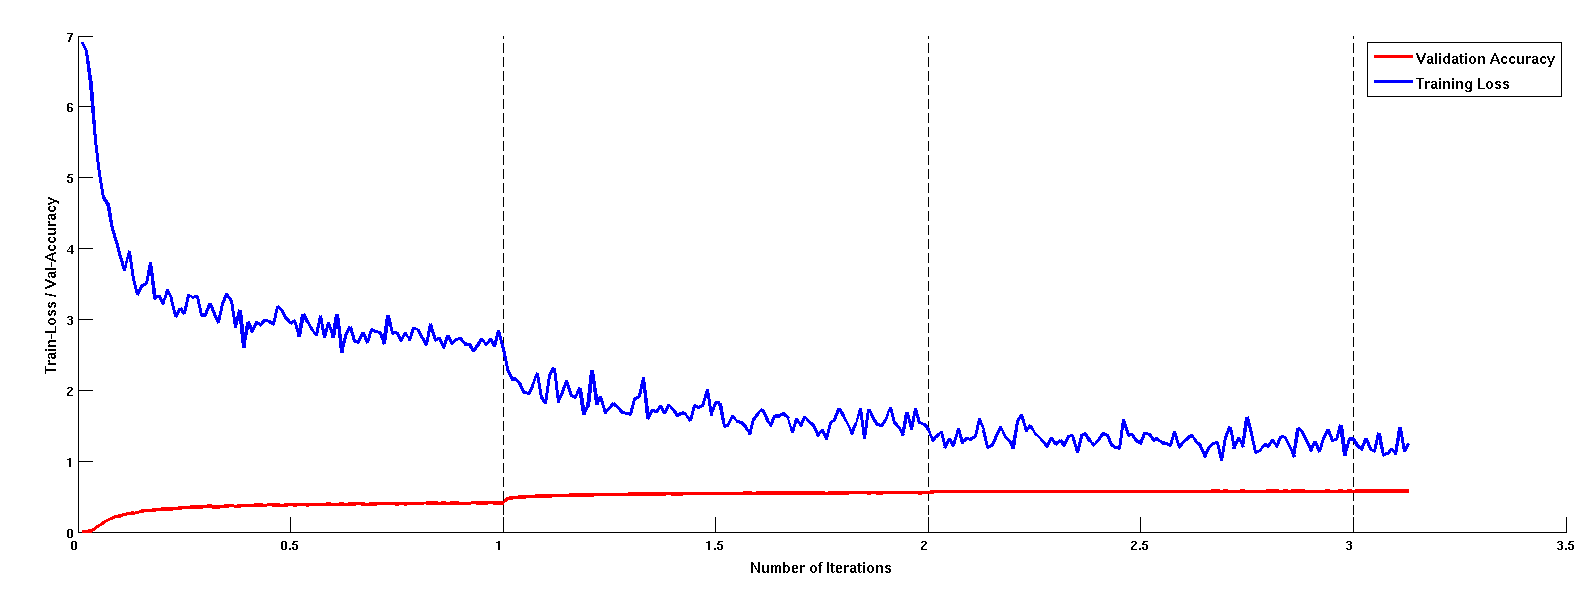
\includegraphics[scale=0.15]{images/training_loss.png}}
\caption{The first row shows conv-1 filters at 5K, 15K and 225K training iteration. The second row shows the evolution of training loss and top-1 accuracy on imagenet ilsvrc-2012 validation set as a function of number of iterations.}
\label{fig:conv1}
\end{figure}

The first thing we try to answer is - if there is an insightful intepretation of the fast intial drop in training loss. Towards this end, we visualized layer 1 filters at different time instances. Surprisingly, we found that within 15K iterations these filters look almost identical to what they would be by the end of the training (See fig \ref{fig:conv1}). This naturally leads us to ask the following questions:
\begin{itemize}
\item {How fast do different layers train? }
\item {Given that discriminative pre-training is helpful, is it the case that there exists a critical point after which learning on imagenet is not helpful for generalizing on other datasets? A "yes" answer to this question will mean that we can speed up the process of fine-tuning.}
\end{itemize}  

In order to objectively answer these questions we evaluated performance of a linear svm classifier learned on features extracted from individual layers on Pascal 2007 classification challenge. The results are summarized in table \ref{table:det-traj-classify}.It is quite surprising to note that by 15K iterations all layers are within 80\% and at 50K iterations within 90\% of there final performance. This strongly indicates that a great portion of training required for generalization happens quite quickly. 

\setlength{\tabcolsep}{4pt}
\begin{table}
\begin{center}
\caption{Variation in classification accuracy (mean-AP) on PASCAL VOC 2007 challenge using features extracted from different layers of Alex-Net as a function of number of iterations.}
\label{table:det-traj-classify}
\begin{tabular}{lcccccccc}
\hline\noalign{\smallskip}
Layer  & 5K & 15K & 25K & 35K & 45K & 95K & 105K & 310K \\
\noalign{\smallskip}
\hline
\noalign{\smallskip}
pool-1 & 23.0 & 24.3 & 24.4 & 24.5 & 24.6 & 24.8 & 24.7 & 25.1\\
pool-2 & 33.7 & 40.4 & 40.9 & 41.8 & 42.0 & 43.2 & 44.0 & 45.0\\
conv-3 & 34.2 & 46.8 & 47.0 & 48.2 & 48.5 & 49.4 & 51.6 & 50.1\\
conv-4 & 33.5 & 49.0 & 48.7 & 50.2 & 50.6 & 51.6 & 54.1 & 54.2\\
pool-5 & 33.0 & 53.4 & 55.0 & 56.8 & 57.4 & 59.2 & 63.5 & 65.6\\
relu-6 & 34.2 & 59.7 & 62.6 & 62.7 & 64.1 & 65.6 & 69.3 & 70.6\\
relu-7 & 30.9 & 61.3 & 64.1 & 65.1 & 65.8 & 67.8 & 71.8 & 73.2\\
\hline
\end{tabular}
\end{center}
\end{table}
\setlength{\tabcolsep}{1.4pt}

Motivated by these observations we trained a 50-50 network (50K iterations on imagenet and finetuned for 50K iterations using the procedure described in sec. \ref{sub:fine-train}) and evaluated its performance on the  Pascal 2007 detection challenge (see table \ref{table:det-trajectory} for results). Consistent with our earlier results we find that this network achieves a surprising performance of 48.6 mean AP points compared to 54.1 achieved by pre-training for 310K iterations. 

\setlength{\tabcolsep}{1pt}
\begin{table}
\begin{center}
\caption{Performance of 50-50 network for detection on pascal-voc-2007 challenge. (l5 is pool-5 and l7 is relu-7)}
\label{table:det-trajectory}
\tiny
\begin{tabular}{l|cccccccccccccccccccc||c}
\hline\noalign{\smallskip}
Feature & aero & bike & bird & boat & bottle & bus & car & cat & chair & cow & table & dog & horse & mbike & person & plant & sheep & sofa & train & tv & mAP \\
\noalign{\smallskip}
\hline
l5(50-50) & 55.2 & 58.4 & 31.0 & 28.8 & 21.0 & 53.5 & 63.6 & 41.0 & 25.4 & 44.7 & 40.9 & 34.9 & 49.5 & 56.9 & 43.8 & 25.2 & 45.3 & 31.2 & 48.7 & 54.4 & 42.7 \\
l5 (full) & 57.8 & 63.9 & 38.8 & 28.0 & 29.0&54.8&66.9&51.3 & 30.5 & 52.1 & 45.2 & 43.2 & 57.3 & 58.8 & 46.0 & 27.2 & 51.2 & 39.3 & 53.3 & 56.6 & 47.6 \\
\hline
l7(50-50) & 58.7 & 64.8 & 38.2 & 34.9 & 25.9 & 59.5 & 69.5 & 46.2 & 28.7 & 52.4 & 45.2 & 44.3 & 57.3 & 63.4 & 52.4 & 28.0 & 51.5 & 34.9 & 56.0 & 59.4 & 48.6 \\
l7(full) & 64.3 & 69.6 & 50.1 & 41.8 & 32.0 & 62.6 & 71.0 & 60.6 & 32.8 & 58.5 & 46.4 & 56.0 & 60.0 & 66.9 & 54.2 & 31.5 & 52.7 & 48.8 & 57.7 & 64.7 & 54.1 \\
\hline
\end{tabular}
\end{center}
\end{table}
\setlength{\tabcolsep}{1.4pt}

** Ross - is this fine to include ? ** 
The take home message from this analysis is that a majority of training happens very early on in the training and a lot of time is spent to achieve the final few points. It is intersting to compare this to learning a SVM where only a few negatives are required for majority of the learning and a lot of time is spent mining for hard-negatives. Almost all the work on training conv-net uses stochastic gradient descent (SGD) for parameter updates. The most widely used version of SGD samples data uniformly, which in light of the above results may not be the optimal strategy. If one could bias the sampling procedure to sample examples analogous to hard-negatives more frequently it may lead to reduction in training time. 

\section{Conclusions}

The paper ends with a conclusion. 

\clearpage\mbox{}Page \thepage\ of the manuscript.

\clearpage

\bibliographystyle{splncs}
\bibliography{egbib}
\end{document}
